\chapter{绪论}

在大数据时代,每天都会产生海量的数据,涵盖各个领域,例如电子商务平台、社交网络、医疗健康等。二分图 (bipartite graph) 作为有效的数据表示方法,能准确描述两个不同群体间的关系,比如电子商务中用户与商品的购买关系,因此被广泛应用于数据建模和分析。其中,极大二分团是二分图中稠密子图,代表两个紧密连接的群体。通过枚举极大二分团,我们可以发现和理解数据中的信息,对知识挖掘、数据分析和智能决策等方面至关重要。因此,极大二分团枚举 (Maximal Biclique Enumeration, MBE) 问题备受研究领域关注。本文主要研究课题是大规模二分图中的极大二分团枚举方法。本章介绍了本课题研究背景,国内外研究现状以及本文的研究内容和组织结构。

\section{研究背景}

随着信息技术的迅猛发展和广泛应用,人类社会正逐渐进入大数据时代,大规模数据的生成和积累已成为一种常态。这些数据涵盖了生活的方方面面,并蕴藏着丰富而有价值的信息。为了充分挖掘和利用这些数据中所蕴含的有效信息,二分图结构被广泛应用于表示两个不同群体之间的联系~\cite{bipartite22}。在二分图中,顶点 (vertex) 代表着不同的数据实体,而边 (edge) 则表示实体之间的关系。二分图结构能够清晰地描述出数据实体之间的交互和连接。具体而言,在二分图中,顶点被划分为两个不同的集合,而同一集合内的顶点之间并未直接相连。例如,在如图\ref{fig:eg_intro}所示的电子商务的场景下,二分图描绘了用户和商品之间的关系,其中顶点可以表示用户或商品,而边则表示购买关系。二分图可以很好地描述了用户与商品之间的关联行为。此外,二分团是指在二分图中形成的一种稠密子图,它代表着数据集中那些紧密连接的群体。以电子商务为例,二分团可以表示同一群用户对同一组商品的产生的批量购买行为。这种紧密的连接揭示了数据中存在的某种规律或者共同特征,为理解群体交易行为提供了一定的线索。而极大二分团是指在二分图中那些独立于其他所有二分团的特殊二分团。它们具有独立性和独特性,不被其他任何二分团所完全包含。识别并枚举二分图中的极大二分团,有助于发现更为细致和确切的群体信息,进一步为深入探究群体行为内部的脉络和联系提供帮助。

\begin{figure} [ht]
  \centering
  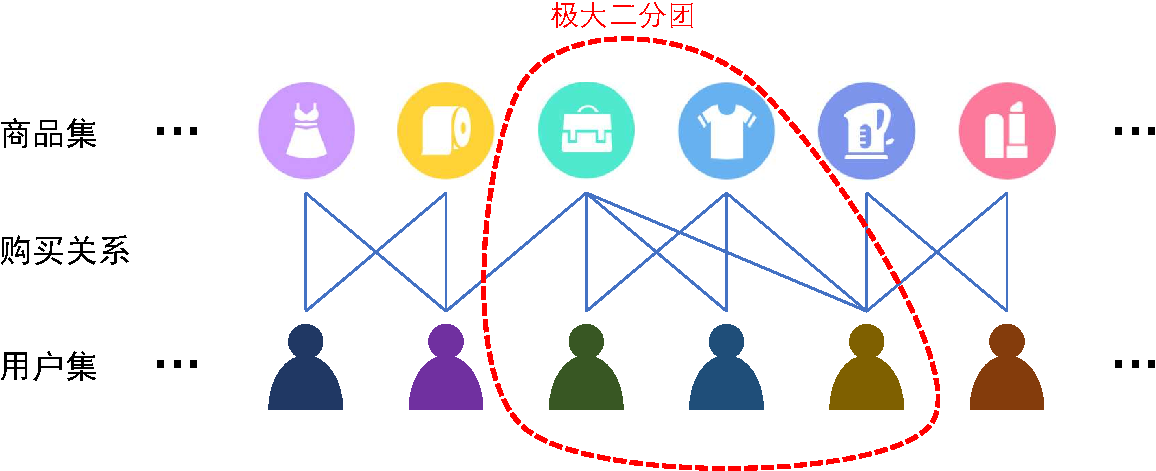
\includegraphics[width=0.7\linewidth]{eg_intro}
  \caption{电子商务场景下的二分图与极大二分团}
  \label{fig:eg_intro}
\end{figure}


极大二分团枚举在二分图数据挖掘方面起到重要辅助作用,具有广泛的应用价值。在电子商务场景下,极大二分团最大程度地描述了用户群体对同组商品的批量购买行为。然而,一些别有用心的商家会通过刷单的方式,雇佣一批用户购买一批目标商品,进而提高目标商品的曝光率,扰乱市场秩序。而极大二分团能够有效地描述此类刷单行为,通过枚举二分团,能够找到所有可疑交易,提升对刷单行为的检出率~\cite{clickfarm21,MEB20,MEB22}。在社交网络场景下,极大二分团最大程度地描述了用户群体的相同兴趣爱好。通过极大二分团枚举,可以更好地辅助社交推荐系统。通过发现用户之间紧密的连接关系,可以推荐给用户其他拥有相似兴趣爱好的用户,从而增加社交互动和用户满意度。同时,极大二分团的枚举还能帮助社交网络平台理解用户行为和需求,优化用户体验,提高平台的粘性和竞争力~\cite{minel06}。在基因分析场景下,极大二分团描述了同一组基因对同一组性状的决定作用。枚举极大二分团能够更好地帮助生物学家理解基因与性状之间的关系。通过分析不同基因之间的连接模式,可以揭示基因之间的相互作用以及它们对性状表现的综合影响。这种基于极大二分团的分析方法能够提供更全面和深入的基因功能研究视角,帮助科学家进一步探索基因调控网络的复杂性和机制。此外,极大二分团的枚举还有助于准确预测基因变异对性状造成的影响,并为疾病研究、遗传工程等领域提供重要的指导意义~\cite{gene22,iMBEA14,protein21}。在图神经网络 (Graph Neural Network, GNN) 领域,极大二分团能够辅助对多个节点数据进行打包,从而加速GNN信息聚合。通过识别和利用极大二分团结构,可以将具有相似特征或者相互关联的节点分为同一个二分团,更高效地进行信息传递和计算,提升图神经网络的训练和推理性能~\cite{PQ21}。总而言之,极大二分团的枚举在电子商务、社交网络、基因分析以及图神经网络等领域都发挥着重要的作用。它能够帮助揭示群体行为、发现不正常的交易行为、辅助推荐系统和加速信息聚合等任务,为相关领域的研究和实践提供有力支持。

\begin{figure} [ht]
  \centering
  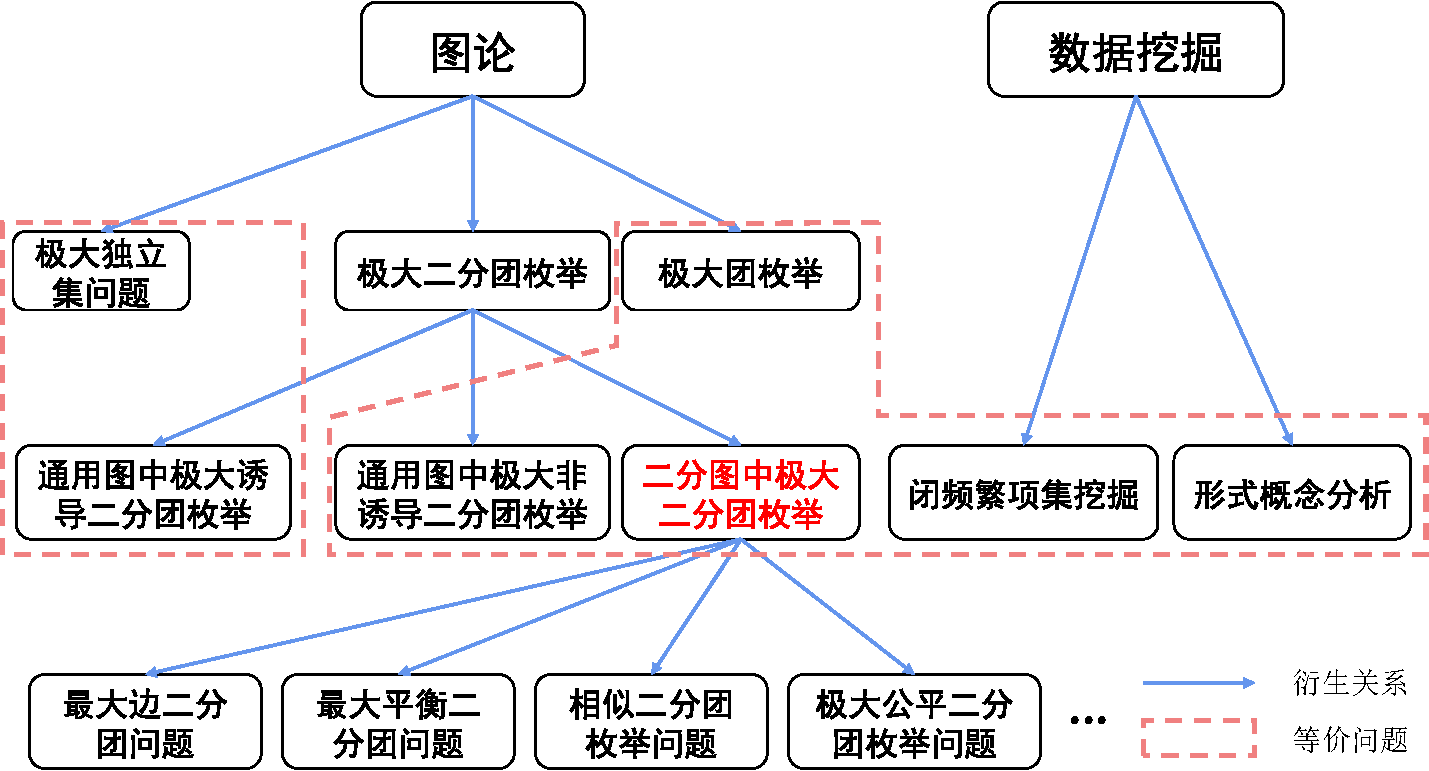
\includegraphics[width=0.8\linewidth]{directory}
  \caption{二分图中极大二分团枚举问题与相关问题的关系图}
  \label{fig:directory}
\end{figure}

同时,极大二分团枚举问题作为图论中的经典组合优化问题,吸引了广泛的研究兴趣。图~\ref{fig:directory}展示了二分图中极大二分团枚举问题与其他相关问题的关系。首先,极大二分团是一种特殊的子图,在通用图中同样存在。通用图中的极大诱导二分团枚举问题可转化为极大独立集问题进行求解~\cite{MBE-induced21};通用图中的极大非诱导二分团枚举问题可转化为二分图中的极大二分团枚举问题进行求解~\cite{Proof09}。考虑到二分图中的极大二分团枚举问题具有广泛的应用价值,本文仅研究二分图中的极大二分团枚举问题。其次,二分图中的极大二分团枚举问题与许多图论领域和数据挖掘领域的经典问题存在一一映射关系。例如极大团枚举问题~\cite{MCE20,MCE-GPU21,MCE22} (Maximal Clique Enumeration, MCE)、闭频繁项挖掘问题~\cite{CFI98,CFI22} (Closed Frequent Itemset Mining, CFI) 和形式概念分析问题~\cite{FCA21,FCA22} (Formal Concept Analysis, FCA)。很多现有的极大二分团枚举方法都受益于这些相关问题的优化思路,部分相关工作将极大二分团枚举问题规约到这些相关问题进行求解。我们将在第~\ref{sec:related}节详细介绍这些方法。相应地,对二分图中极大二分团枚举问题的优化研究间接地为解决这些问题提供了思路。最后,随着二分图中极大二分团问题研究的深入,近年来,极大二分团枚举方法被应用于最大边二分团寻找~\cite{MEB20,MEB22} (Maximum Edge Biclique Search, MEB) 和最大平衡二分团寻找~\cite{MBB21} (Maximum Balanced Biclique Search, MBB) 等问题中,并衍生出相似二分团枚举问题~\cite{SimilarMBE22}、(p,q)二分团枚举问题\cite{PQ21}和公平极大二分团枚举问题~\cite{FairMBE23}等相关问题。这些问题都基于极大二分团枚举算法进行实现和探索,为进一步扩展和拓展极大二分团的应用领域提供了可能性。总之,二分图中极大二分团枚举问题在图论研究中具有重要地位。对于该问题的深入研究将会对其他相关问题的研究起到辐射带动作用。

% 同时,极大二分团枚举问题作为图论中的经典组合优化问题,吸引了广泛的研究兴趣。探索极大二分团枚举问题不仅可以深入理解其本身的性质和特点,还可以为其他相关问题的解决提供线索和启示。极大二分团枚举问题与一些其他问题之间存在紧密的联系。例如,它可以与极大团枚举问题~\cite{MCE20,MCE-GPU21,MCE22}、闭频繁项挖掘问题~\cite{FCI98,FCI22}和形式概念分析问题~\cite{FCA21,FCA22}相互映射。对极大二分团枚举问题的优化研究间接地为解决这些问题提供了思路。此外,最大边二分团寻找~\cite{MEB20,MEB22}和最大平衡二分团寻找~\cite{MBB21}等问题是在所有极大二分团中寻找特定类型的二分团。现有的研究工作已经证明,高效的极大二分团枚举算法可以直接加速这些问题的求解过程~\cite{ooMBE22}。除此之外,近年来,极大二分团枚举问题还产生了许多变种问题,如相似二分团枚举问题~\cite{SimilarMBE22}、(p,q)二分团枚举问题\cite{PQ21}和公平极大二分团枚举问题~\cite{FairMBE23}等。这些问题都基于极大二分团枚举算法进行实现和探索,为进一步扩展和拓展极大二分团的应用领域提供了可能性。总之,极大二分团枚举问题在图论研究中具有重要地位,其对于其他相关问题解决思路的提供和衍生问题的产生,使其成为一个值得深入研究的课题。

然而,极大二分团枚举面临着严峻的挑战。首先,极大二分团枚举问题是一种NP-hard问题,即在多项式时间内无法高效地解决。随着二分图顶点数量的增加,极大二分团问题的求解难度呈指数级增长~\cite{MICA04}。这意味着在大规模二分图中进行极大二分团枚举的计算复杂度非常高。举个例子,具有18万个顶点和44万条边的二分图Github中,其内部极大二分团的数量已经超过了5534万个~\cite{konect}。据统计数据显示,目前最优的极大二分团枚举算法ooMBEA~\cite{ooMBE22}。在Github数据集上执行极大二分团枚举任务时,产生的无效枚举数量是极大二分团数量的26倍,这表明仍然存在巨大的优化空间。其次,在大数据时代,二分图的规模仍在不断增加。以电子商务为例,根据中国商务部的电子商务报告~\cite{ECommerceReport},2022年全国电子商务交易额达到43.83万亿元。按可比口径计算,与上一年相比增长了3.5\%。据统计,仅在2020年,阿里巴巴企业一天内的交易次数已超过1亿次~\cite{MEB20}。因此,在这种情况下,如何设计高效的极大二分团枚举算法,并快速地在大规模二分图中找到所需的极大二分团,面临着极大的挑战。最后,相较于其他子图枚举问题,极大二分团枚举问题的特点之一是每个极大二分团的顶点数量较多且不固定,导致该问题更加复杂和不规则~\cite{Irregularity12}。在图枚举算法中,每个被枚举子图的计算时间与子图内顶点数量呈正相关关系,因此极大二分团枚举问题中每个极大二分团的顶点数量差异会导致计算时长上的差异。特别是当枚举涉及到包含许多顶点的极大二分团时,其计算所需时间会显著增加,从而进一步加剧了负载不均衡的问题,严重影响了并行性能。为了提高极大二分团枚举算法的效率和可扩展性,我们需要探索新的方法和技术来解决这些挑战。

综上所述,极大二分团枚举问题在图论领域扮演着基础问题的角色,并且在数据挖掘中具有重要的辅助作用和实际应用价值。然而,在处理大规模二分图时,极大二分团枚举算法面临严峻的挑战,在枚举空间、数据结构以及并行扩展等方面仍存在很大的优化空间。因此,探索在大规模二分图中高效解决极大二分团枚举问题的方法成为一项重要的研究课题。

\section{国内外研究现状}
\label{sec:related}

作为图论中的基础问题,关于极大二分团枚举问题的研究最早可追溯到1962年~\cite{MBE62}。在过去的几十年中,国内外学者对二分图中的极大二分团枚举问题进行了深入的研究,并取得了一系列重要的成果。

早期的极大二分团枚举问题研究中,学者们尝试通过结合其他相关研究问题的经验来解决该问题。其中,Makino等人~\cite{Makino04}观察到二分图上的极大二分团枚举问题可以通过图膨胀的方式映射到通用图上的极大团枚举问题进行求解。具体地,他们将二分图中的每个顶点集合内的任意两个顶点添加一条边,从而膨胀原二分图中的每个极大二分团,使其对应于膨胀后通用图中的一个极大团,然后利用已有的极大团枚举方法进行求解~\cite{MCEparallel20,MCE20,MCE22}。然而,这种方法并不实用,因为它在二分图的基础上增加了大量非必要的边,导致了该问题的计算难度增加,严重影响了计算性能。另一方面,Zaki等人~\cite{CFI98}注意到事务数据库中的闭频繁项与二分图中的极大二分团存在一一对应的关系。基于这个对应关系,Li等人~\cite{correspondence05}指出了数据挖掘领域中一些经典算法对于极大二分团枚举问题的解决具有帮助作用,例如FPclose~\cite{fpclose04}和LCM~\cite{lcm04}等算法。通过计算闭频繁项集,可以得到极大二分团中的一个顶点集合,进而计算另一个顶点集合以构成二分团。Li等人还在LCM算法的基础上提出了LCM-MBC算法来进行极大二分团枚举。然而,对于闭频繁项挖掘算法而言,在大规模事务性数据库中将支持度设置为1进行闭频繁项挖掘是非常困难的~\cite{iMBEA14}。另外,Gaume等人~\cite{fcambe10}指出二分图中的极大二分团与形式概念分析问题中的形式概念之间存在平行关系。因此,现有的形式概念分析相关工作~\cite{FCA15,FCA21,FCA22}可以应用于极大二分团枚举问题的求解。然而,这些形式概念分析方法主要适用于二进制数据的分析~\cite{FCA15},即源数据通过位图方式存储并采用位运算进行计算。由于现实中的二分图往往是稀疏的,采用位图存储方式会带来大量的内存开销,因此目前前沿的形式概念分析算法只能在小规模图上应用~\cite{FCA21,FCA22},在处理大规模二分图时会导致超出内存限制的问题。Alexe等人~\cite{MICA04}通过共识算法枚举了所有可能的候选极大二分团,但该算法的时间复杂度较高。综上所述,直接应用其他相关研究问题的方法,不适用于大规模二分图上的极大二分团枚举问题的求解。

% 早期的极大二分团枚举问题研究中,大量的研究工作借鉴其他相关研究问题的经验,根据极大二分团枚举问题与其他问题的联系来解决极大二分团枚举问题。(1) Makino等人~\cite{Makino04}观察到二分图上的极大二分团枚举问题可以通过图膨胀的方式映射到通用图上的极大团枚举问题进行求解。具体地,对于二分图中的两个顶点集合,该方法为每个顶点集合内的任意两个顶点添加一条边,因此,原二分图中的每个极大二分团对应膨胀后通用图中的一个极大团,然后用已有的极大团枚举方法进行求解~\cite{MCEparallel20,MCE20,MCE22}。然而,该方法是不实用的,因为它在二分图基础上增加了大量的非必要的边,增加了该问题的计算难度,严重影响计算性能。(2) Zaki等人~\cite{CFI98}注意到事务数据库中的闭频繁项和二分图中的极大二分团存在一一对应的关系。根据这个对应关系,Li等人~\cite{correspondence05}指出数据挖掘领域的经典算法,如FPclose~\cite{fpclose04},LCM~\cite{lcm04}等,对极大二分团枚举问题有帮助作用。利用对闭频繁项集的计算,可以得到极大二分团中的一个顶点集,进而计算另一个顶点集构成二分团。Li等人~\cite{lcmmbc07}在LCM算法的基础上提出LCM-MBC算法用于极大二分团枚举。然而,对于闭频繁项挖掘算法而言,在大的事务性数据库中,将支持度设置为1进行闭频繁项挖掘是很困难的~\cite{iMBEA14}。(3) Gaume等人~\cite{fcambe10}指出二分图中的极大二分团与形式概念分析问题中的形式概念存在平行关系。因此,现有的形式概念分析相关的工作~\cite{FCA,FCA21,FCA22}可以用于极大二分团枚举问题的求解。然而,形式概念分析相关的工作主要在二进制数据上展开~\cite{FCA15},即源数据通过位图方式存储并以位运算的方式开展计算。由于现实中的二分图是稀疏的,位图存储方式会带来大量的内存开销,这导致前沿的形式概念分析算法只能在小图上进行~\cite{FCA21,FCA22},在大规模二分图中会带来内存超过限制的问题。

\begin{figure} [ht]
  \centering
  \vspace{0.3 in}
  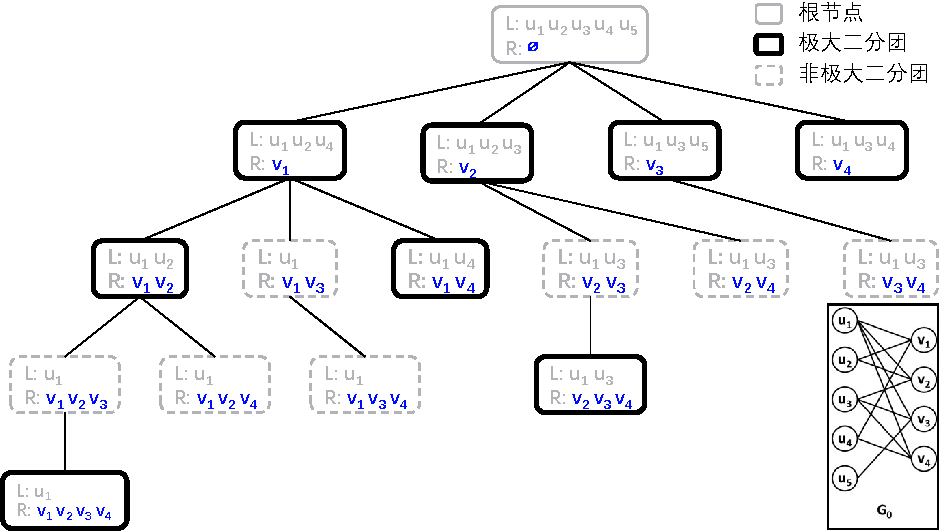
\includegraphics[width=0.9\linewidth]{se_tree}
  \vspace{0.2 in}
  \caption{极大二分团枚举算法中的集合枚举树}
  \label{fig:se}
\end{figure}

早期的极大二分团枚举问题研究中,学者们尝试通过结合其他相关研究问题的经验来解决该问题。其中,Makino等人~\cite{Makino04}观察到二分图上的极大二分团枚举问题可以通过图膨胀的方式映射到通用图上的极大团枚举问题进行求解。具体地,他们将二分图中的每个顶点集合内的任意两个顶点添加一条边,从而膨胀原二分图中的每个极大二分团,使其对应于膨胀后通用图中的一个极大团,然后利用已有的极大团枚举方法进行求解~\cite{MCEparallel20,MCE20,MCE22}。然而,这种方法并不实用,因为它在二分图的基础上增加了大量非必要的边,导致了该问题的计算难度增加,严重影响了计算性能。另一方面,Zaki等人~\cite{CFI98}注意到事务数据库中的闭频繁项与二分图中的极大二分团存在一一对应的关系。基于这个对应关系,Li等人~\cite{correspondence05}指出了数据挖掘领域中一些经典算法对于极大二分团枚举问题的解决具有帮助作用,例如FPclose~\cite{fpclose04}和LCM~\cite{lcm04}等算法。通过计算闭频繁项集,可以得到极大二分团中的一个顶点集合,进而计算另一个顶点集合以构成二分团。Li等人还在LCM算法的基础上提出了LCM-MBC算法来进行极大二分团枚举。然而,对于闭频繁项挖掘算法而言,在大规模事务性数据库中将支持度设置为1进行闭频繁项挖掘是非常困难的~\cite{iMBEA14}。另外,Gaume等人~\cite{fcambe10}指出二分图中的极大二分团与形式概念分析问题中的形式概念之间存在平行关系。因此,现有的形式概念分析相关工作~\cite{FCA15,FCA21,FCA22}可以应用于极大二分团枚举问题的求解。然而,这些形式概念分析方法主要适用于二进制数据的分析~\cite{FCA15},即源数据通过位图方式存储并采用位运算进行计算。由于现实中的二分图往往是稀疏的,采用位图存储方式会带来大量的内存开销,因此目前前沿的形式概念分析算法只能在小规模图上应用~\cite{FCA21,FCA22},在处理大规模二分图时会导致超出内存限制的问题。Alexe等人~\cite{MICA04}通过共识算法枚举了所有可能的候选极大二分团,但该算法的时间复杂度较高。综上所述,直接应用其他相关研究问题的方法在大规模二分图中进行极大二分团枚举是低效的。

目前,主流且高效的极大二分团枚举算法基于集合枚举树~\cite{SEtree92} (Set-Enumeration-Tree, SE-tree) 的数据结构实现。集合枚举树是一种用于系统地枚举特定集合幂集的工具。给定一个二分图$G(U, V, E)$,其中$U$和$V$表示两个不相交的顶点集合,$E$表示边集合,$E \subseteq U \times V$。该类枚举算法首先利用集合枚举树生成$V$集合的幂集,然后将$V$集合的幂集中的集合扩展成二分团,输出其中的全部极大二分团。图~\ref{fig:se}展示了一棵用于极大二分团枚举的集合枚举树。集合枚举树首先将$V$集合的幂集生成到每个树节点的$R$集合中(标记为蓝色),然后每个节点将所有与$R$内顶点完全相连的顶点作为顶点的$L$集合,最后枚举其中所有的极大二分团$(L,R)$。2006年,Liu等人提出MineLMBC算法~\cite{minel06},首次引入集合枚举树,采用分治法求解极大二分团枚举问题。此后,基于枚举树的极大二分团枚举方法得到了不断优化。为了减少枚举空间、提升计算效率,研究者们相继提出了不同的优化技术。Zhang等人提出iMBEA算法~\cite{iMBEA14},采用了顶点度数升序排序和排除顶点集等技术,以减少枚举时间。Das等人提出FMBE算法~\cite{parMBE18},通过主动计算顶点的二跳邻居作为候选顶点集合,加速了枚举过程。Abidi等人提出PMBE算法~\cite{PMBE20},借鉴了极大团枚举问题中的枢纽顶点思路,利用枢纽顶点进行剪枝。Chen等人提出ooMBEA算法~\cite{ooMBE22},引入了单边排序和批量枢纽顶点剪枝等技术,进一步减少了枚举时间。为了进一步提高效率,研究者们设计了并行极大二分团枚举算法。Mukherjee等人利用MapReduce框架实现了分布式极大二分团枚举算法CDFS~\cite{mapreduceMBE16}。然而,大量的跨节点通信开销导致该算法效率较低。Das等人提出多核算法ParMBE~\cite{parMBE18},但该算法的并行性受限于计算核心数量的限制。此外,国内的He等人提出优化的sMBEA算法~\cite{MBEHe18},Qin等人利用栈的特性实现了EMBE算法~\cite{MBEQin20}。然而,与其他主流算法(如FMBE、PMBE、ooMBEA等)相比,这两个算法存在较大的性能差距。综上所述,基于极大枚举树的
极大二分团枚举方法最适合解决大规模二分图中的极大二分团枚举问题,但仍存在较大的优化空间。

除了上述工作外,其他研究对输入的二分图以及输出的极大二分团进行了特定的约束。Damaschke等人~\cite{Damaschke14}提出了一种输出敏感的极大二分团枚举算法,该算法基于二分图中顶点度数的倾斜分布。然而,该算法对输入二分图的要求较为苛刻,只适用于特定情况下的求解,并不能很好地适用于一般二分图。Shaham等人~\cite{Shaham16}提出基于聚类的方法,在二分团搜索的子空间中利用蒙特卡洛方法获取随机种子并将其扩展为极大二分团。然而,这种方法只能枚举部分的极大二分团,无法覆盖所有可能的极大二分团。针对动态二分图,Ma等人~\cite{Ma22}提出了一种有效保持最大二分团性质的框架。该框架可以在动态变化的二分图上进行高效的极大二分团枚举。另外,近年来的一些研究工作定义了特殊类型的极大二分团,并对这些特殊类型的二分团进行枚举。例如,Yao等人~\cite{SimilarMBE22}定义了极大相似二分团,Sun等人~\cite{Sun22}定义了极大平衡有符号二分团,Yin等人~\cite{FairMBE23}定义了极大二分团的公平性。这些算法都是基于极大二分团枚举算法,并在枚举过程中对输出进行适当的约束和限制,以适应特定的问题需求。综上所述,极大二分团枚举在这些研究中发挥着基础性作用。


% 除此之外,其他的二分图上的极大二分团枚举相关的算法在问题的输入输出上进行了特定的约束。Damaschke等人~\cite{Damaschke14}利用二分图中顶点度数的倾斜分布提出了输出敏感的极大二分团枚举算法,但是该算法对输入二分图的要求苛刻,不适用于一般二分图的求解。Shaham等人~\cite{Shaham16}提出了一种二分团子空间聚类算法,通过蒙特卡洛方法获取随机种子扩展为极大二分团,但是该方法只能枚举部分的极大二分团。Ma等人~\cite{Ma22}针对动态二分图,提出了在动态二分图上有效保持最大二分图的框架。近年来,部分研究工作对定义了许多特殊的极大二分团并对自定义的二分团进行枚举,如Yao等人~\cite{SimilarMBE22}定义了极大相似二分团,Sun等人~\cite{Sun22}定义了极大平衡有符号二分团,Yin等人~\cite{FairMBE23}定义了极大二分团的公平性。这些算法都是基于极大二分团枚举算法,对输出进行适当约束实现的。

% 给定一个二分图$G(U, V, E)$,其中$U$和$V$表示两个不相交的顶点集合,$E$表示边集合,$E \subseteq U \times V$。该类枚举算法首先利用集合枚举树生成$V$集合的幂集,之后将$V$集合的幂集中的集合扩展成二分团,保留并输出其中的全部极大二分团。具体的生成过程我们将在第~\ref{ch:intro} 章进行详细描述。2006年,Liu等人提出MineLMBC~\cite{minel06},首次引入集合枚举树用于求解极大二分团枚举问题。2007年,Liu等人基于高效的频繁项挖掘算法LCM提出LCM-MBC~\cite{lcmmbc07},证明了闭频繁项挖掘问题与极大二分团枚举问题的一一对应关系,将极大二分团问题与闭频繁项挖掘问题联系起来。此后,基于枚举树的极大二分团枚举方法的优化层出不穷。表~\ref{tbl:sota}中整理了近年来基于集合枚举树实现的极大二分团枚举方法的相关优化工作。

\section{本文主要研究内容与结构}

针对大规模二分图中的极大二分团问题,本文首先观察到现有工作在枚举空间、数据结构、并性扩展呈现低效性。随后,本文系统地从枚举空间优化、数据结构选择以及并行扩展三个方面分别开展研究,并分别形成三个高效的针对大规模二分图的极大二分团枚举问题的解决方案。具体地研究内容如结构如图~\ref{fig:outline}所示:

\begin{figure} [ht]
  \vspace{0.2 in}
  \centering
  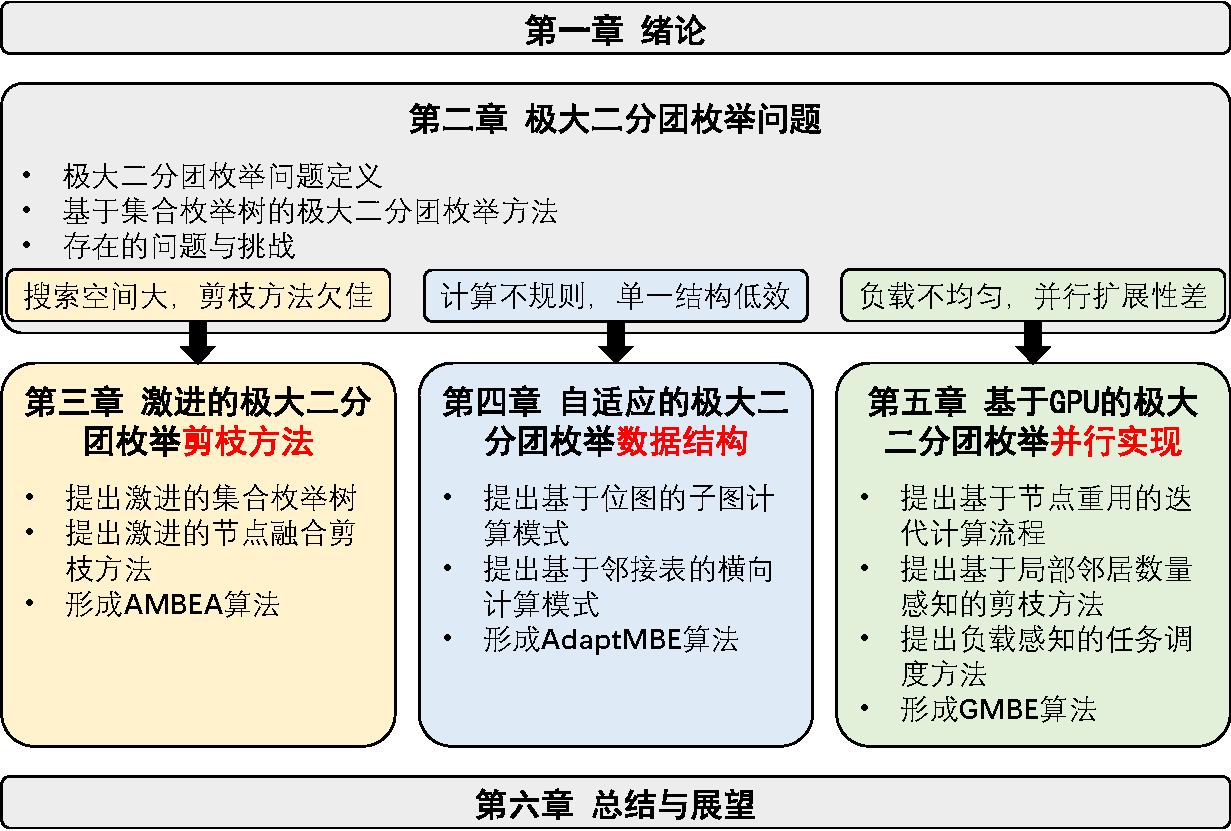
\includegraphics[width=\linewidth]{outline}
  \vspace{0.15 in}
  \caption{本文主要研究内容与结构}
  \label{fig:outline}
\end{figure}

第一章作为绪论,介绍了大规模二分图中的极大二分团枚举问题在数据挖掘领域和图论领域中重要作用,以及国内外的相关研究工作现状。

第二章详细地介绍了二分图中的极大二分团枚举问题。本章首先给出问题的正式定义与相关符号定义,然后介绍了主流的基于集合枚举树的极大二分团枚举方法,最后指出现有方法现有方法在大规模二分图中进行极大二分团枚举所呈现的低效性问题,具体包含枚举空间优化、数据结构选择以及并行扩展三个方面的挑战。针对这些挑战,本文在第三至第五章分别提出三种不同的解决方案。

第三章介绍了激进的极大二分团枚举剪枝方法,以优化枚举空间提升枚举性能。针对现有的极大二分团枚举方法在大规模二分图中仍会产生大量非极大二分团的问题,本章提出了一种激进的集合枚举树和一种激进的顶点融合剪枝方法,并结合上述两种方法形成AMBEA算法。实验证明,AMBEA算法在大规模二分图中的枚举性能优于现有方法,得益于其高效的剪枝性能。

第四章介绍了自适应的极大二分团枚举数据结构,采用混合数据结构以提升枚举性能。针对现有极大二分团枚举方法采用单一数据结构所带来的低效性问题,本章针对位图和邻接表两种数据结构分别提出了不同的计算模式,并结合这两种计算模式形成AdaptMBE算法。实验证明,基于混合数据结构的AdaptMBE枚举算法比现有方法更具计算优势。

第五章介绍了基于GPU的极大二分团枚举并行实现,利用GPU的大量计算核心极大地缩短了枚举时间。针对现有极大二分团枚举算法只能在基于CPU的计算系统中运行且受限于计算核心数量的计算性能问题,本章提出了首个基于GPU的极大二分团枚举算法。针对在GPU上进行极大二分团枚举所面临的内存不足、线程分歧以及负载不均问题,本章提出了基于节点重用的迭代计算流程、基于节点重用的迭代计算流程和负载感知的任务调度方法,最终形成GMBE算法。实验证明,基于GPU的GMBE算法在性能上显著优于现有基于CPU的方法,具有更短的执行时间。

第六章对全文进行总结,并展望未来的研究方向。



